\fancyhf{}
\fancyhead[LE,RO]{\bfseries\textsf{53}}
\fancyhead[RE,LO]{\small\bfseries\textsf{MỤC 1.4}\quad\textmd{Hàm số mũ}}

\noindent
\begin{multicols}{2}
\fontsize{8.5pt}{10.8pt}\selectfont
\setlength{\abovedisplayskip}{3pt}
\setlength{\belowdisplayskip}{3pt}

% Biểu tượng công nghệ [T] và đồ thị
\providecommand{\techsymbol}{\tikz[baseline=-0.5ex]{\node[draw=stewartcyan,fill=stewartcyan!10,inner sep=1.2pt,line width=0.6pt,rounded corners=0.5pt]{\fontsize{6.5pt}{6.5pt}\selectfont\bfseries\color{stewartcyan}T};}}
\providecommand{\graphsymbol}{\tikz[baseline=-0.5ex]{\draw[stewartcyan,line width=0.7pt] (0,0) rectangle (0.28,0.22); \draw[stewartcyan,line width=0.7pt] (0.04,0.05) .. controls (0.1,0.18) and (0.18,0.04) .. (0.24,0.17);}}

% BÀI 27
\noindent\techsymbol\ \textbf{27.} Một nhà nghiên cứu đang cố gắng xác định thời gian nhân đôi đối với một quần thể vi khuẩn \textit{Giardia lamblia}. Ông bắt đầu nuôi cấy trong một dung dịch dinh dưỡng và ước tính số lượng vi khuẩn sau mỗi bốn giờ. Dữ liệu của ông được thể hiện trong bảng bên dưới.

\begin{center}
\resizebox{\linewidth}{!}{%
\renewcommand{\arraystretch}{1.25}
\begin{tabular}{|>{\columncolor[HTML]{DDE5ED}}l|c|c|c|c|c|c|c|}
\hline
Thời gian (giờ) & 0 & 4 & 8 & 12 & 16 & 20 & 24 \\
\hline
\begin{tabular}{@{}l@{}}Số lượng vi khuẩn\\[-2pt](CFU/mL)\end{tabular} & 37 & 47 & 63 & 78 & 105 & 130 & 173 \\
\hline
\end{tabular}%
}
\end{center}

\begin{enumerate}[label=(\alph*),leftmargin=1.5em,itemsep=1pt,topsep=1pt]
    \item Vẽ biểu đồ phân tán của dữ liệu.
    \item Sử dụng máy tính cầm tay hoặc máy vi tính để tìm một đường cong hàm mũ $f(t) = a \cdot b^t$ mô hình hóa số lượng vi khuẩn sau $t$ giờ.
    \item Vẽ đồ thị của mô hình từ phần (b) cùng với biểu đồ phân tán ở phần (a). Sử dụng đồ thị này để ước tính thời gian cần thiết để số lượng vi khuẩn tăng gấp đôi.
\end{enumerate}

\begin{center}
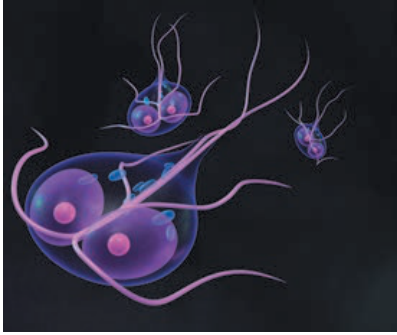
\includegraphics[width=0.82\linewidth]{images/p0088_raster_1.png}\\[3pt]
\textit{G. lamblia}
\end{center}

% BÀI 28
\noindent\techsymbol\ \textbf{28.} Bảng bên dưới cho biết dân số của Hoa Kỳ, tính theo triệu người, trong các năm 1900--2010. Hãy sử dụng máy tính vẽ đồ thị (hoặc máy vi tính) có tính năng hồi quy hàm mũ để mô hình hóa dân số Hoa Kỳ kể từ năm 1900. Sử dụng mô hình đó để ước tính dân số vào năm 1925 và dự đoán dân số vào năm 2020.

\begin{center}
\renewcommand{\arraystretch}{1.12}
\begin{tabular}{|>{\centering\arraybackslash}m{2.2cm}|>{\centering\arraybackslash}m{2.8cm}|}
\hline
\rowcolor[HTML]{DDE5ED} \textbf{Năm} & \textbf{Dân số} \\
\hline
1900 & 76 \\
1910 & 92 \\
1920 & 106 \\
1930 & 123 \\
1940 & 131 \\
1950 & 150 \\
1960 & 179 \\
1970 & 203 \\
1980 & 227 \\
1990 & 250 \\
2000 & 281 \\
2010 & 310 \\
\hline
\end{tabular}
\end{center}

% BÀI 29
\noindent\textbf{29.} Một mẻ nuôi cấy vi khuẩn bắt đầu với 500 vi khuẩn và tăng gấp đôi số lượng sau mỗi nửa giờ.
\begin{enumerate}[label=(\alph*),leftmargin=1.5em,itemsep=1pt,topsep=1pt]
    \item Có bao nhiêu vi khuẩn sau 3 giờ?
    \item Có bao nhiêu vi khuẩn sau $t$ giờ?
    \item Có bao nhiêu vi khuẩn sau 40 phút?
    \item[\graphsymbol\ (d)] Vẽ đồ thị hàm số biểu diễn số lượng quần thể và ước tính thời gian để quần thể đạt đến 100.000 cá thể.
\end{enumerate}

% BÀI 30
\noindent\textbf{30.} Một quần thể sóc xám được đưa vào một khu vực nhất định cách đây 18 năm. Các nhà sinh học quan sát thấy rằng quần thể tăng gấp đôi sau mỗi 6 năm, và hiện tại số lượng là 600 con.
\begin{enumerate}[label=(\alph*),leftmargin=1.5em,itemsep=1pt,topsep=1pt]
    \item Số lượng sóc ban đầu là bao nhiêu?
    \item Số lượng sóc dự kiến sau $t$ năm kể từ khi được đưa vào là bao nhiêu?
    \item Ước tính số lượng sóc dự kiến sau 10 năm nữa tính từ thời điểm hiện tại.
\end{enumerate}

% BÀI 31
\noindent\textbf{31.} Trong Ví dụ 4, tải lượng vi-rút $V$ của bệnh nhân là 76,0 bản sao RNA trên mỗi mL sau một ngày điều trị. Hãy sử dụng đồ thị của $V$ trong Hình 11 để ước tính lượng thời gian cần thiết thêm để tải lượng vi-rút giảm xuống còn một nửa lượng đó.

% BÀI 32
\noindent\textbf{32.} Sau khi rượu được hấp thu hoàn toàn vào cơ thể, nó sẽ được chuyển hóa. Giả sử sau khi uống một số đồ uống có cồn vào đầu buổi tối, nồng độ cồn trong máu (BAC) của bạn vào lúc nửa đêm là 0,14 g/dL. Sau 1,5 giờ, chỉ số BAC của bạn giảm xuống còn một nửa lượng này.
\begin{enumerate}[label=(\alph*),leftmargin=1.5em,itemsep=1pt,topsep=1pt]
    \item Tìm một mô hình hàm mũ cho chỉ số BAC của bạn sau $t$ giờ tính từ nửa đêm.
    \item[\graphsymbol\ (b)] Vẽ đồ thị hàm BAC của bạn và sử dụng đồ thị để xác định khi nào BAC đạt mức giới hạn pháp lý là 0,08 g/dL.
\end{enumerate}
\vspace{1pt}
{\fontsize{7.5pt}{9.5pt}\selectfont\textit{Nguồn:} Phỏng theo P. Wilkinson và cộng sự, ``Pharmacokinetics of Ethanol after Oral Administration in the Fasting State,'' \textit{Journal of Pharmacokinetics and Biopharmaceutics} 5 (1977): 207--24.\par}

% BÀI 33
\noindent\graphsymbol\ \textbf{33.} Nếu bạn vẽ đồ thị của hàm số
\[
f(x) = \frac{1 - e^{1/x}}{1 + e^{1/x}}
\]
bạn sẽ thấy rằng dường như $f$ là một hàm số lẻ. Hãy chứng minh điều đó.

% BÀI 34
\noindent\graphsymbol\ \textbf{34.} Hãy vẽ đồ thị của một số hàm số trong họ hàm
\[
f(x) = \frac{1}{1 + ae^{bx}}
\]
với $a > 0$. Đồ thị thay đổi như thế nào khi $b$ thay đổi? Đồ thị thay đổi như thế nào khi $a$ thay đổi?

% BÀI 35
\noindent\graphsymbol\ \textbf{35.} Hãy vẽ đồ thị của một số hàm số trong họ hàm
\[
f(x) = \frac{a}{2}\left(e^{x/a} + e^{-x/a}\right)
\]
với $a > 0$. Đồ thị thay đổi như thế nào khi $a$ tăng lên?

\end{multicols}